% Options for packages loaded elsewhere
\PassOptionsToPackage{unicode}{hyperref}
\PassOptionsToPackage{hyphens}{url}
%
\documentclass[
]{article}
\usepackage{amsmath,amssymb}
\usepackage{iftex}
\ifPDFTeX
  \usepackage[T1]{fontenc}
  \usepackage[utf8]{inputenc}
  \usepackage{textcomp} % provide euro and other symbols
\else % if luatex or xetex
  \usepackage{unicode-math} % this also loads fontspec
  \defaultfontfeatures{Scale=MatchLowercase}
  \defaultfontfeatures[\rmfamily]{Ligatures=TeX,Scale=1}
\fi
\usepackage{lmodern}
\ifPDFTeX\else
  % xetex/luatex font selection
\fi
% Use upquote if available, for straight quotes in verbatim environments
\IfFileExists{upquote.sty}{\usepackage{upquote}}{}
\IfFileExists{microtype.sty}{% use microtype if available
  \usepackage[]{microtype}
  \UseMicrotypeSet[protrusion]{basicmath} % disable protrusion for tt fonts
}{}
\makeatletter
\@ifundefined{KOMAClassName}{% if non-KOMA class
  \IfFileExists{parskip.sty}{%
    \usepackage{parskip}
  }{% else
    \setlength{\parindent}{0pt}
    \setlength{\parskip}{6pt plus 2pt minus 1pt}}
}{% if KOMA class
  \KOMAoptions{parskip=half}}
\makeatother
\usepackage{xcolor}
\usepackage[margin=1in]{geometry}
\usepackage{color}
\usepackage{fancyvrb}
\newcommand{\VerbBar}{|}
\newcommand{\VERB}{\Verb[commandchars=\\\{\}]}
\DefineVerbatimEnvironment{Highlighting}{Verbatim}{commandchars=\\\{\}}
% Add ',fontsize=\small' for more characters per line
\usepackage{framed}
\definecolor{shadecolor}{RGB}{248,248,248}
\newenvironment{Shaded}{\begin{snugshade}}{\end{snugshade}}
\newcommand{\AlertTok}[1]{\textcolor[rgb]{0.94,0.16,0.16}{#1}}
\newcommand{\AnnotationTok}[1]{\textcolor[rgb]{0.56,0.35,0.01}{\textbf{\textit{#1}}}}
\newcommand{\AttributeTok}[1]{\textcolor[rgb]{0.13,0.29,0.53}{#1}}
\newcommand{\BaseNTok}[1]{\textcolor[rgb]{0.00,0.00,0.81}{#1}}
\newcommand{\BuiltInTok}[1]{#1}
\newcommand{\CharTok}[1]{\textcolor[rgb]{0.31,0.60,0.02}{#1}}
\newcommand{\CommentTok}[1]{\textcolor[rgb]{0.56,0.35,0.01}{\textit{#1}}}
\newcommand{\CommentVarTok}[1]{\textcolor[rgb]{0.56,0.35,0.01}{\textbf{\textit{#1}}}}
\newcommand{\ConstantTok}[1]{\textcolor[rgb]{0.56,0.35,0.01}{#1}}
\newcommand{\ControlFlowTok}[1]{\textcolor[rgb]{0.13,0.29,0.53}{\textbf{#1}}}
\newcommand{\DataTypeTok}[1]{\textcolor[rgb]{0.13,0.29,0.53}{#1}}
\newcommand{\DecValTok}[1]{\textcolor[rgb]{0.00,0.00,0.81}{#1}}
\newcommand{\DocumentationTok}[1]{\textcolor[rgb]{0.56,0.35,0.01}{\textbf{\textit{#1}}}}
\newcommand{\ErrorTok}[1]{\textcolor[rgb]{0.64,0.00,0.00}{\textbf{#1}}}
\newcommand{\ExtensionTok}[1]{#1}
\newcommand{\FloatTok}[1]{\textcolor[rgb]{0.00,0.00,0.81}{#1}}
\newcommand{\FunctionTok}[1]{\textcolor[rgb]{0.13,0.29,0.53}{\textbf{#1}}}
\newcommand{\ImportTok}[1]{#1}
\newcommand{\InformationTok}[1]{\textcolor[rgb]{0.56,0.35,0.01}{\textbf{\textit{#1}}}}
\newcommand{\KeywordTok}[1]{\textcolor[rgb]{0.13,0.29,0.53}{\textbf{#1}}}
\newcommand{\NormalTok}[1]{#1}
\newcommand{\OperatorTok}[1]{\textcolor[rgb]{0.81,0.36,0.00}{\textbf{#1}}}
\newcommand{\OtherTok}[1]{\textcolor[rgb]{0.56,0.35,0.01}{#1}}
\newcommand{\PreprocessorTok}[1]{\textcolor[rgb]{0.56,0.35,0.01}{\textit{#1}}}
\newcommand{\RegionMarkerTok}[1]{#1}
\newcommand{\SpecialCharTok}[1]{\textcolor[rgb]{0.81,0.36,0.00}{\textbf{#1}}}
\newcommand{\SpecialStringTok}[1]{\textcolor[rgb]{0.31,0.60,0.02}{#1}}
\newcommand{\StringTok}[1]{\textcolor[rgb]{0.31,0.60,0.02}{#1}}
\newcommand{\VariableTok}[1]{\textcolor[rgb]{0.00,0.00,0.00}{#1}}
\newcommand{\VerbatimStringTok}[1]{\textcolor[rgb]{0.31,0.60,0.02}{#1}}
\newcommand{\WarningTok}[1]{\textcolor[rgb]{0.56,0.35,0.01}{\textbf{\textit{#1}}}}
\usepackage{longtable,booktabs,array}
\usepackage{calc} % for calculating minipage widths
% Correct order of tables after \paragraph or \subparagraph
\usepackage{etoolbox}
\makeatletter
\patchcmd\longtable{\par}{\if@noskipsec\mbox{}\fi\par}{}{}
\makeatother
% Allow footnotes in longtable head/foot
\IfFileExists{footnotehyper.sty}{\usepackage{footnotehyper}}{\usepackage{footnote}}
\makesavenoteenv{longtable}
\usepackage{graphicx}
\makeatletter
\def\maxwidth{\ifdim\Gin@nat@width>\linewidth\linewidth\else\Gin@nat@width\fi}
\def\maxheight{\ifdim\Gin@nat@height>\textheight\textheight\else\Gin@nat@height\fi}
\makeatother
% Scale images if necessary, so that they will not overflow the page
% margins by default, and it is still possible to overwrite the defaults
% using explicit options in \includegraphics[width, height, ...]{}
\setkeys{Gin}{width=\maxwidth,height=\maxheight,keepaspectratio}
% Set default figure placement to htbp
\makeatletter
\def\fps@figure{htbp}
\makeatother
\setlength{\emergencystretch}{3em} % prevent overfull lines
\providecommand{\tightlist}{%
  \setlength{\itemsep}{0pt}\setlength{\parskip}{0pt}}
\setcounter{secnumdepth}{5}
\ifLuaTeX
  \usepackage{selnolig}  % disable illegal ligatures
\fi
\usepackage{bookmark}
\IfFileExists{xurl.sty}{\usepackage{xurl}}{} % add URL line breaks if available
\urlstyle{same}
\hypersetup{
  pdftitle={COMPASS Synopitic Porewater Nutrients 2022-2024},
  pdfauthor={Fausto Machado-Silva \& Roberta B. Peixoto},
  hidelinks,
  pdfcreator={LaTeX via pandoc}}

\title{COMPASS Synopitic Porewater Nutrients 2022-2024}
\author{Fausto Machado-Silva \& Roberta B. Peixoto}
\date{2026-03-31}

\begin{document}
\maketitle

{
\setcounter{tocdepth}{2}
\tableofcontents
}
\newpage

\subsection{Run Information}\label{run-information}

\begin{Shaded}
\begin{Highlighting}[]
\CommentTok{\#set the run date \& user name }
\NormalTok{  run\_date }\OtherTok{\textless{}{-}} \StringTok{"03/06/2026"}
\NormalTok{  sample\_year }\OtherTok{\textless{}{-}} \StringTok{"2023"}
\NormalTok{  sample\_month }\OtherTok{\textless{}{-}} \StringTok{"Feb"}
\NormalTok{  user }\OtherTok{\textless{}{-}} \StringTok{"Fausto Machado{-}Silva"}
\NormalTok{  QAQC\_by }\OtherTok{\textless{}{-}} \StringTok{"Fausto Machado{-}Silva"}

\CommentTok{\#identify the files you want to read in }
  \CommentTok{\# read in as a list to accommodate multiple runs in a month}
\NormalTok{  data\_files }\OtherTok{\textless{}{-}} \FunctionTok{c}\NormalTok{(}\StringTok{"Raw Data/COMPASS\_Box7\_MonMon\_NUTR\_noPO4\_385{-}465\_Feb2023\_JB.csv"}\NormalTok{, }
                  \StringTok{"Raw Data/Redo\_COMPASS\_Box7\_MonMon\_PO4.NOx.SO4\_385{-}465\_Feb2023\_JB.csv"}
\NormalTok{                  )}

\NormalTok{  data\_list }\OtherTok{\textless{}{-}} \FunctionTok{lapply}\NormalTok{(data\_files, read.csv)}
\NormalTok{  data\_file }\OtherTok{\textless{}{-}}\NormalTok{ dplyr}\SpecialCharTok{::}\FunctionTok{bind\_rows}\NormalTok{(data\_list)}

  
\CommentTok{\# Define the file path for QAQC log file {-} NO Need to change just check year }
\NormalTok{  file\_path }\OtherTok{\textless{}{-}} \StringTok{"Raw Data/COMPASS\_Box7\_MonMon\_Nutrients\_QAQC\_Std\_curves\_log.csv"}
\NormalTok{  final\_path }\OtherTok{\textless{}{-}} \StringTok{"Processed Data/COMPASS\_Box7\_MonMon\_Nutrients.csv"}

\CommentTok{\#record any notes about the run or anything other info here: }
\NormalTok{  run\_notes }\OtherTok{\textless{}{-}} \StringTok{"Two run dates: (1st) NOx, NO2, NH4, SO4, (2nd) NOx, SO4 and PO4"} \CommentTok{\#Add notes from QAQC}
  
\CommentTok{\#Set up file path for metadata }
  \CommentTok{\#downloaded metadata csv {-} downloaded from Google drive as csv for this year}
\NormalTok{  Raw\_Metadata }\OtherTok{=} \StringTok{"Raw Data/COMPASS\_LE\_Nutrient\_SampleLog.csv"}
  
\CommentTok{\#Set up file path for standard curves }
  \CommentTok{\#downloaded metadata csv {-} downloaded from Google drive as csv for this year}
\NormalTok{  st\_curve }\OtherTok{=} \StringTok{"Raw Data/COMPASS\_LE\_Nutrients\_St\_curve\_Box7\_NOx\_NO2\_NH4\_SO4.csv"}

  \FunctionTok{cat}\NormalTok{(run\_notes)}
\end{Highlighting}
\end{Shaded}

\begin{verbatim}
## Two run dates: (1st) NOx, NO2, NH4, SO4, (2nd) NOx, SO4 and PO4
\end{verbatim}

\#\#Setup

\#\#Read in metadata and create similar sample IDs for matching to
samples

\newpage

\#\#Import Data \& Clean

\#\#Assessing standard Curves

\begin{verbatim}
##      Test  ID Absorbance  Conc Target    Error     Unit Run_Date
## 1 Sulfate  S1     0.0020  0.40      0       NA mg SO4/L 3/5/2025
## 2 Sulfate *90     0.0224  3.71      5 -25.8058 mg SO4/L 3/5/2025
## 3 Sulfate S91     0.0545  9.31     10  -6.9269 mg SO4/L 3/5/2025
## 4 Sulfate S92     0.0826 14.61     15  -2.5840 mg SO4/L 3/5/2025
## 5 Sulfate S93     0.1109 20.34     20   1.7250 mg SO4/L 3/5/2025
## 6 Sulfate S94     0.1591 31.00     30   3.3181 mg SO4/L 3/5/2025
\end{verbatim}

\subsection{Plot standard curves}\label{plot-standard-curves}

\begin{verbatim}
## `geom_smooth()` using formula = 'y ~ x'
\end{verbatim}

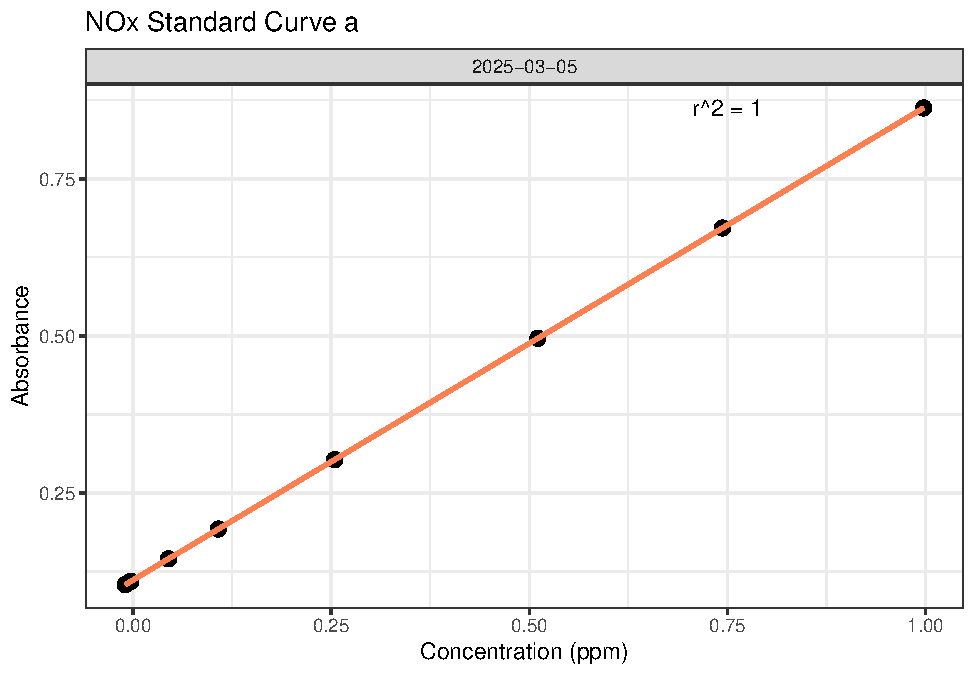
\includegraphics{COMPASS_LE_Synoptic_NUTR_2022-2024_Box_7_files/figure-latex/Plot Standard Curves-1.pdf}

\begin{verbatim}
## `geom_smooth()` using formula = 'y ~ x'
\end{verbatim}

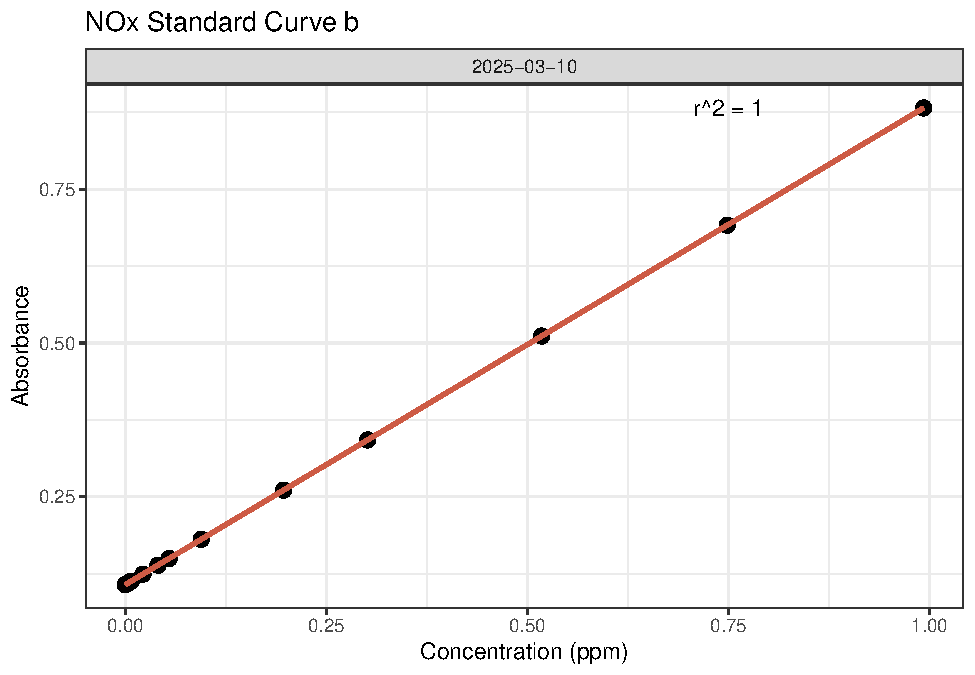
\includegraphics{COMPASS_LE_Synoptic_NUTR_2022-2024_Box_7_files/figure-latex/Plot Standard Curves-2.pdf}

\begin{verbatim}
## `geom_smooth()` using formula = 'y ~ x'
\end{verbatim}

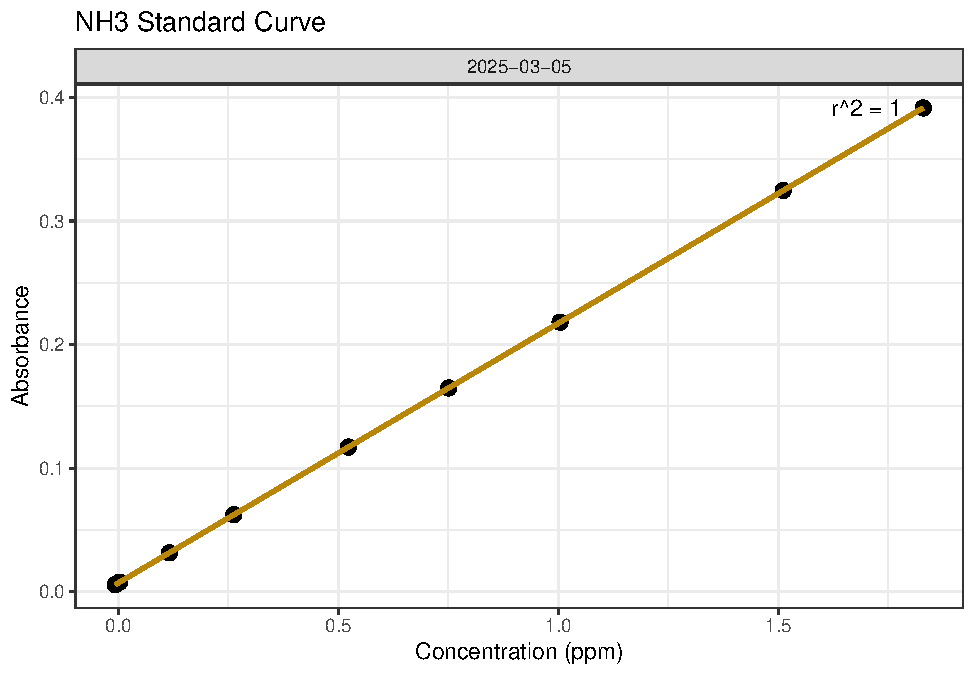
\includegraphics{COMPASS_LE_Synoptic_NUTR_2022-2024_Box_7_files/figure-latex/Plot Standard Curves-3.pdf}

\begin{verbatim}
## `geom_smooth()` using formula = 'y ~ x'
\end{verbatim}

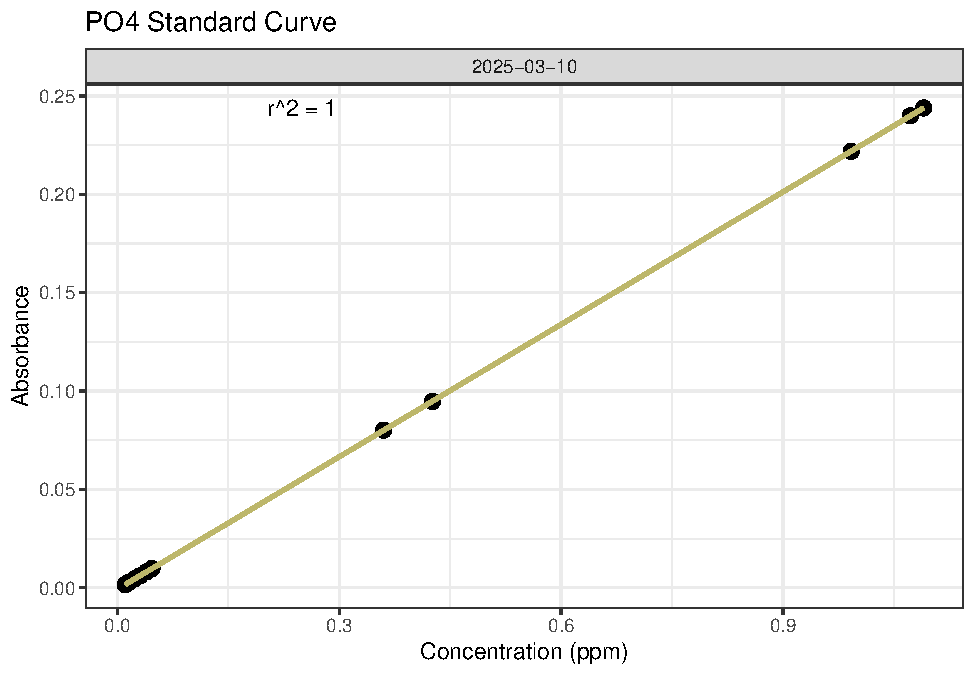
\includegraphics{COMPASS_LE_Synoptic_NUTR_2022-2024_Box_7_files/figure-latex/Plot Standard Curves-4.pdf}
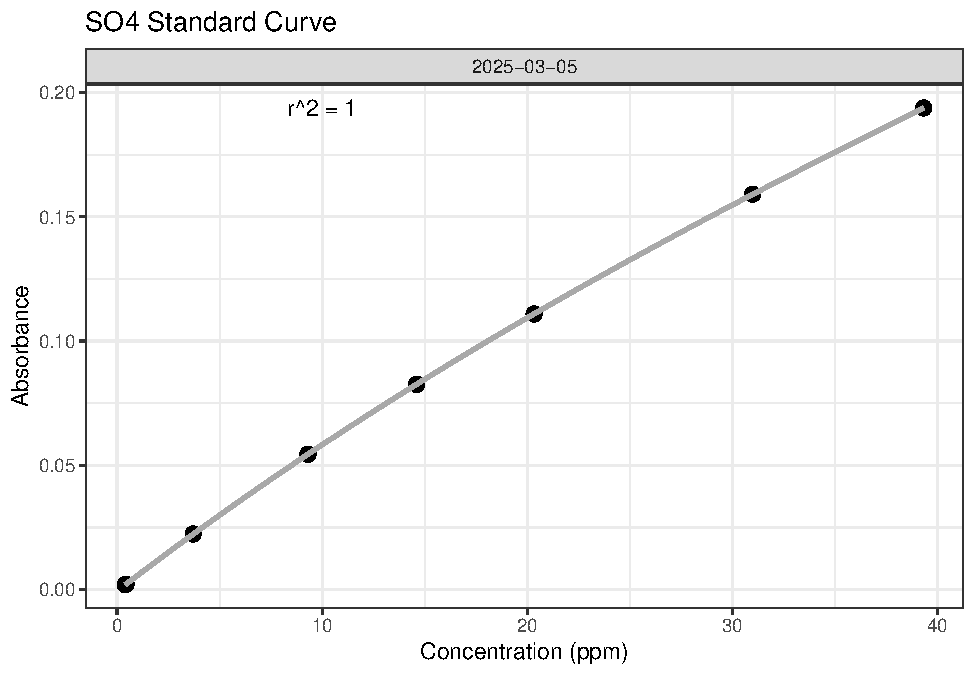
\includegraphics{COMPASS_LE_Synoptic_NUTR_2022-2024_Box_7_files/figure-latex/Plot Standard Curves-5.pdf}
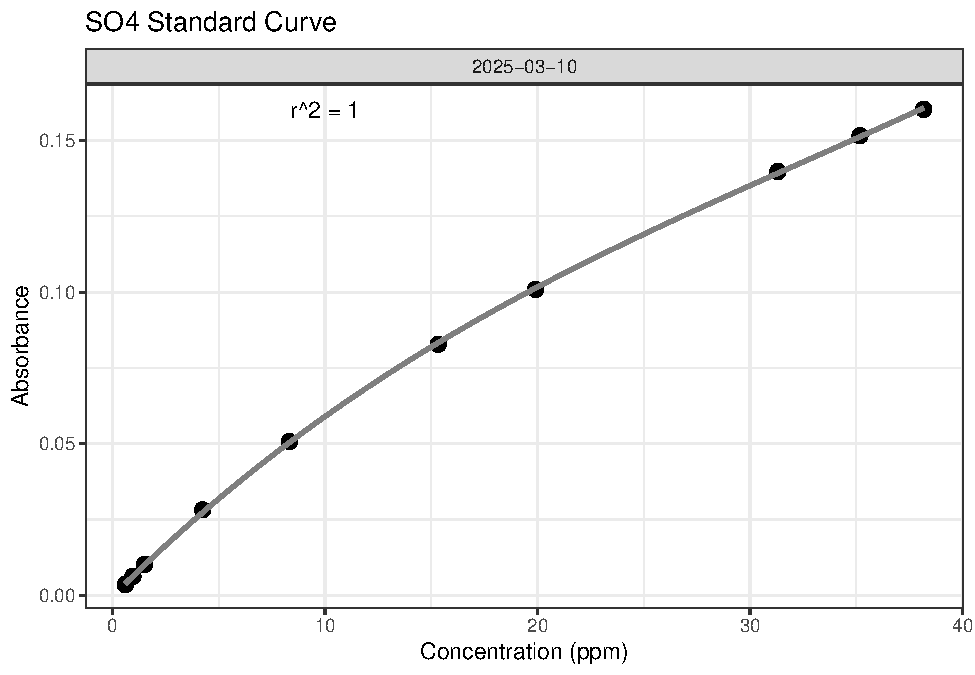
\includegraphics{COMPASS_LE_Synoptic_NUTR_2022-2024_Box_7_files/figure-latex/Plot Standard Curves-6.pdf}

\begin{verbatim}
## `geom_smooth()` using formula = 'y ~ x'
\end{verbatim}

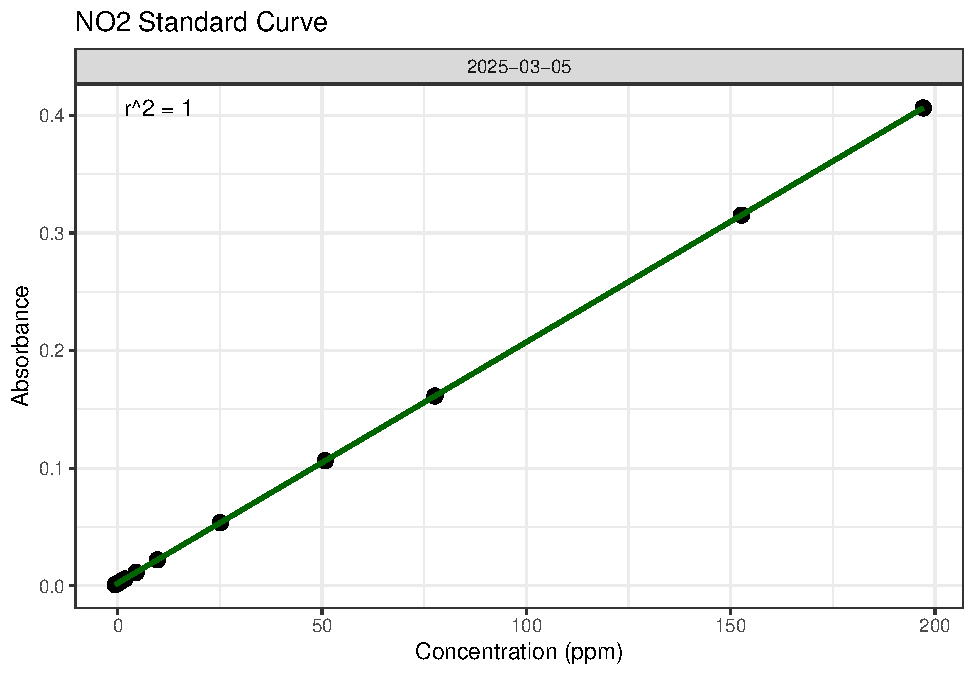
\includegraphics{COMPASS_LE_Synoptic_NUTR_2022-2024_Box_7_files/figure-latex/Plot Standard Curves-7.pdf}

\begin{verbatim}
## [1] "NOx Curve r2 GOOD - PROCEED"
\end{verbatim}

\begin{verbatim}
## [1] "NOx Curve r2 GOOD - PROCEED"
\end{verbatim}

\begin{verbatim}
## [1] "NH3 Curve r2 GOOD - PROCEED"
\end{verbatim}

\begin{verbatim}
## [1] "PO4 Curve r2 GOOD - PROCEED"
\end{verbatim}

\begin{verbatim}
## [1] "SO4 Curve r2 GOOD - PROCEED"
\end{verbatim}

\begin{verbatim}
## [1] "SO4 Curve r2 GOOD - PROCEED"
\end{verbatim}

\begin{verbatim}
## [1] "NO2 Curve r2 GOOD - PROCEED"
\end{verbatim}

\begin{verbatim}
## [1] "QAQC log file exists and has been read into the code."
\end{verbatim}

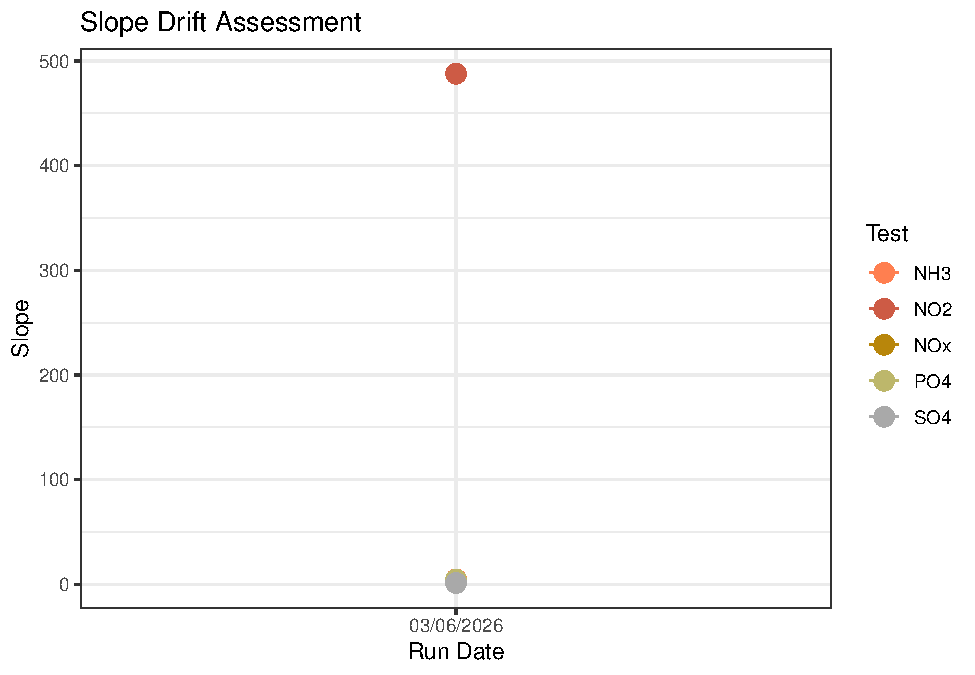
\includegraphics{COMPASS_LE_Synoptic_NUTR_2022-2024_Box_7_files/figure-latex/Plot Standard Curves-8.pdf}

\begin{longtable}[]{@{}lr@{}}
\caption{Average Slope by Analyte}\tabularnewline
\toprule\noalign{}
Test & avg\_slope \\
\midrule\noalign{}
\endfirsthead
\toprule\noalign{}
Test & avg\_slope \\
\midrule\noalign{}
\endhead
\bottomrule\noalign{}
\endlastfoot
NH3 & 4.761 \\
NO2 & 487.805 \\
NOx & 1.304 \\
PO4 & 4.455 \\
SO4 & 1.304 \\
\end{longtable}

\newpage

\#\#Dilution Corrections - ensure the latest dilution is kept

\begin{verbatim}
## Duplicated samples: 2 ppm SO4, Field Blank, 1 ppm NOx Standard
\end{verbatim}

\begin{verbatim}
## 
## WARNING: Duplicated samples with NO dilution (possible input error):
## # A tibble: 6 x 4
##   Test            Sample_Name        n_dups any_dilution
##   <chr>           <chr>               <int> <lgl>       
## 1 "Ammonia (PPS)" Field Blank             3 FALSE       
## 2 "Nitrate (NOx)" 1 ppm NOx Standard      6 FALSE       
## 3 "Nitrate (NOx)" Field Blank             6 FALSE       
## 4 "Nitrite"       Field Blank             3 FALSE       
## 5 "Phosphate "    Field Blank             3 FALSE       
## 6 "Sulfate"       2 ppm SO4               3 FALSE
\end{verbatim}

\subsection{Check NOx Reduction
Efficiency}\label{check-nox-reduction-efficiency}

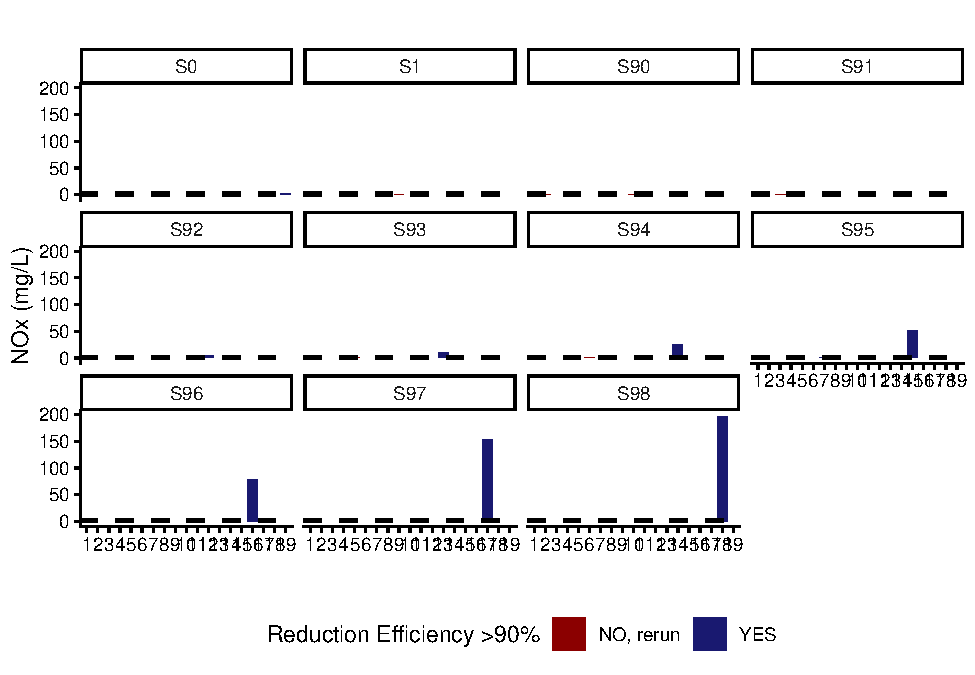
\includegraphics{COMPASS_LE_Synoptic_NUTR_2022-2024_Box_7_files/figure-latex/Assess reduction Efficiency-1.pdf}

\begin{verbatim}
## [1] "Mean NOx Reduction Efficiency >95% - PROCEED"
\end{verbatim}

\begin{verbatim}
## [1] 2750.881
\end{verbatim}

\newpage

\subsection{Analyze the Check
Standards}\label{analyze-the-check-standards}

\begin{verbatim}
## [1] "NOx Check Standard RSD within Range - PROCEED"
\end{verbatim}

\begin{verbatim}
## [1] "NH3 Check Standard RSD within Range - PROCEED"
\end{verbatim}

\begin{verbatim}
## [1] "PO4 Check Standard RSD within Range - PROCEED"
\end{verbatim}

\begin{verbatim}
## [1] "SO4 Check Standard RSD within Range - PROCEED"
\end{verbatim}

\begin{verbatim}
## [1] "NO2 Check Standard RSD within Range - PROCEED"
\end{verbatim}

\includegraphics{COMPASS_LE_Synoptic_NUTR_2022-2024_Box_7_files/figure-latex/Check Standards-1.pdf}

\begin{verbatim}
## [1] ">60% of NOx Check Standards are within range of expected concentration - PROCEED"
\end{verbatim}

\begin{verbatim}
## [1] "<60% of NH3 Check Standards are within range of expected concentration - REASSESS"
\end{verbatim}

\begin{verbatim}
## [1] "<60% of PO4 Check Standards are within range of expected concentration - REASSESS"
\end{verbatim}

\begin{verbatim}
## [1] "<60% of SO4 Check Standards are within range of expected concentration - REASSESS"
\end{verbatim}

\begin{verbatim}
## [1] ">60% of NO2 Check Standards are within range of expected concentration - PROCEED"
\end{verbatim}

\newpage

\subsection{Analyze Blanks}\label{analyze-blanks}

\begin{verbatim}
## [1] ">60% of NOx Blanks are below the lower 25% quartile of samples or 1/2 detection limit - PROCEED"
\end{verbatim}

\begin{verbatim}
## [1] ">60% of NH3 Blanks are below the lower 25% quartile of samples - PROCEED"
\end{verbatim}

\begin{verbatim}
## [1] ">60% of PO4 Blanks  are below the lower 25% quartile of samples- PROCEED"
\end{verbatim}

\begin{verbatim}
## [1] ">60% of SO4 Blanks  are below the lower 25% quartile of samples- PROCEED"
\end{verbatim}

\begin{verbatim}
## [1] ">60% of NO2 Blanks  are below the lower 25% quartile of samples- PROCEED"
\end{verbatim}

\includegraphics{COMPASS_LE_Synoptic_NUTR_2022-2024_Box_7_files/figure-latex/Analyze Blanks-1.pdf}

\begin{longtable}[]{@{}lr@{}}
\caption{Mean Concentration of Blanks}\tabularnewline
\toprule\noalign{}
Test & Blank\_Mean\_Conc \\
\midrule\noalign{}
\endfirsthead
\toprule\noalign{}
Test & Blank\_Mean\_Conc \\
\midrule\noalign{}
\endhead
\bottomrule\noalign{}
\endlastfoot
NOx & -0.0047 \\
NH3 & -0.0031 \\
PO4 & 0.0121 \\
SO4 & 0.5441 \\
NO2 & 1.4590 \\
\end{longtable}

\newpage

\#\#Sample Flagging - Within range of standard curve

\#\#Pull out sample id information

\subsection{Check to see if samples run match metadata \& merge
info}\label{check-to-see-if-samples-run-match-metadata-merge-info}

\begin{verbatim}
## Check Sample IDs with Metadata
\end{verbatim}

\begin{verbatim}
## All sample IDs are present in metadata.
\end{verbatim}

\newpage

\subsection{Visualize data}\label{visualize-data}

\begin{verbatim}
## Visualize Data
\end{verbatim}

\includegraphics{COMPASS_LE_Synoptic_NUTR_2022-2024_Box_7_files/figure-latex/Visualize data-1.pdf}
\includegraphics{COMPASS_LE_Synoptic_NUTR_2022-2024_Box_7_files/figure-latex/Visualize data-2.pdf}
\includegraphics{COMPASS_LE_Synoptic_NUTR_2022-2024_Box_7_files/figure-latex/Visualize data-3.pdf}
\includegraphics{COMPASS_LE_Synoptic_NUTR_2022-2024_Box_7_files/figure-latex/Visualize data-4.pdf}
\includegraphics{COMPASS_LE_Synoptic_NUTR_2022-2024_Box_7_files/figure-latex/Visualize data-5.pdf}

\#\#Export Processed Data

\#end

\end{document}
